\chapter{บทนำ}
\thispagestyle{empty}
\label{chapter:introduction}

\section{ที่มาและความสำคัญ}
    {\Company} เป็นบริษัทขายปลีกที่จำหน่ายสินค้าและให้บริการที่เกี่ยวข้องกับการก่อสร้าง ตกแต่ง ต่อเติม ซ่อมแซม ปรับปรุง อาคาร บ้าน และที่อยู่อาศัยแบบครบวงจร
    แต่หากว่า โฮมโปรหน้าร้านบางสาขาอาจจะไม่มีสินค้าที่ลูกค้าต้องการอยู่เพราะขนาดของสาขาของโฮมโปรมีหลายขนาดตั้งแต่ร้านขนาดเล็กที่ตั้งอยู่ในห้างสรรพสินค้าของเจ้าอื่น
    ไปจนถึงตั้งแยกออกมาเป็นห้างสรรพสินค้าขนาดใหญ่ของตนเองจึงทำให้สินค้าที่มีอยู่ไม่สามารถแสดงได้ทั้งหมดตามขนาดโฮมโปรจึงจัดทำแอปพลิเคชัน E-Catalog ขึ้นมา
    แอปพลิเคชัน E-Catalog คือแอปพลิเคชันในการสนับสนุนการขายของพนักงานสาขาในการที่จะแสดงสินค้าที่โฮมโปรมีแต่สาขาที่ลูกค้าอยู่ไม่มีได้ยกตัวอย่างเช่น โฮมโปร
    สาขา ประชาชื่น ไม่มีแอร์รุ่นที่ลูกค้าต้องการพนักงานขายของสาขาสามารถแสดงรูปตัวอย่างสินค้าและคุณสมบัติของสินค้าผ่านแอปพลิเคชันให้ลูกค้าดูว่าตรงกับความต้องการลูกค้าหรือไม่และแสดง
    ถึงสาขาที่มี แอร์อยู่ได้อีกทั้งยังสามารถสั่งจองสินค้านั้นจากสาขาที่มีผ่านทางแอปพลิเคชันได้เลยเพียงแค่กรอกเบอร์โทรศัพท์ และ แอปพลิเคชันสามารถใช้ในการช่วยขายสินค้าที่เกี่ยวข้องกัน
    ให้กับลูกค้าเพิ่มเติมได้ เช่น ลูกค้าเลือกซื้อประตูพนักงานสาขาสามารถแสดงลูกบิดที่ดูเหมาะสมเข้ากับประตูนั้นได้ เป็นต้น
    เพื่อป้องกันข้อผิดพลาดก่อนนำแอปพลิเคชันไปใช้จริงต้องทดสอบเพื่อสังเกตหาข้อผิดพลาดทุกครั้งโดยแต่ละครั้งหากตัวแอปพลิเคชันเกิดการแก้ไขแม้ว่าจะมากหรือน้อยก็ตาม
    เพราะการแก้ไขแต่ละครั้งอาจจะส่งผลกระทบกับส่วนอื่นๆของแอปพลิเคชันได้ แต่จะเสียแรงงานและเวลากับการทดสอบได้หากเกิดการแก้ไขบ่อยครั้ง
    ดังนั้นบริษัท โฮมโปรดักส์ เซ็นเตอร์ จํากัด (มหาชน) จึงได้เล็งเห็นถึงความสําคัญของการทดสอบ
    แอปพลิเคชันแบบอัตโนมัติ จึงให้นักศึกษาปฏิบัติงานโครงการทวิภาคีสถาบันเทคโนโลยีพระจอมเกล้าเจ้าคุณทหารลาดกระบัง นาย เสฎฐวุฒิ ไม้สนธิ์ ทำการทดสอบโดยการเขียนชุดคำสั่งทดสอบอัตโนมัติ (automate testing) ให้ใช้คู่กับ AWS Device Farm
    ในการพัฒนาชุดคำสั่งทดสอบอัตโนมัติเพื่อลดระยะเวลาและแรงงานในการทดสอบแอปพลิเคชันแบบเดิม

\section{วัตถุประสงค์}
    \begin{enumerate}
        \item เพื่อพัฒนาทักษะของตนเองในการพัฒนาชุดคำสั่งทดสอบอัตโนมัติ
        \item เพื่อลดข้อผิดพลาดจากการทดสอบแอปพลิเคชันแบบ Manual
        \item ลดเวลาการทดสอบและส่งมอบแอปพลิเคชันได้รวดเร็วขึ้น
        \item เพื่อเป็นต้นแบบในการทดสอบแอปพลิเคชันตัวอื่นของบริษัทต่อไป
    \end{enumerate}

\section{ประวัติ และรายละเอียดสถานประกอบการ}
    \subsection{ชื่อ และสถานที่ตั้งของสถานประกอบการ}
        {\Company}

        ที่อยู่ {\Company} สำนักงานใหญ่

        {\Address}
    \subsection{ประวัติความเป็นมาของสถานประกอบการ}
        บมจ. โฮม โปรดักส์ เซ็นเตอร์ จดทะเบียนจัดตั้งขึ้นเมื่อวันที่ 27 มิถุนายน 2538 โดยเป็นการร่วมลงทุนของ บมจ. แลนด์แอนด์เฮ้าส์ และ บมจ. ควอลิตี้เฮ้าส์ บริษัทฯ เริ่มต้นเปิดดำเนินการที่สาขารังสิตในเดือนกันยายน 2539 เป็นแห่งแรก โดยใช้ชื่อทางการค้าว่า “โฮมโปร” (HomePro)
        บริษัทฯ ได้จดทะเบียนแปรสภาพเป็นบริษัทมหาชนในวันที่ 29 พฤษภาคม 2544 ด้วยทุนจดทะเบียนเริ่มต้น 150 ล้านบาท ต่อมาได้จดทะเบียนเป็นบริษัทรับอนุญาตในตลาดหลักทรัพย์แห่งประเทศไทยในวันที่ 30 ตุลาคม 2544 โดยใช้ชื่อย่อหลักทรัพย์ว่า “HMPRO”
        ในวันที่ 26 พฤษภาคม 2548 บริษัทฯ ได้จดทะเบียนจัดตั้งบริษัท มาร์เก็ต วิลเลจ จำกัด โดยมีวัตถุประสงค์เพื่อบริหารพื้นที่ให้เช่า พร้อมกับให้บริการทางด้านสาธารณูปโภค เริ่มต้นดำเนินการในไตรมาสแรก ปี 2549 ที่โครงการ “หัวหิน มาร์เก็ต วิลเลจ” (Hua-Hin Market Village)
        และในปี 2549 บริษัทฯ ได้ถูกคัดเลือกให้เป็นหลักทรัพย์ในกลุ่ม SET100
        ในปี 2553 บริษัทฯ ได้รับคัดเลือกให้เป็นหลักทรัพย์ในกลุ่ม SET 50  และได้เปิดดำเนินการครบ 15 ปี มีสาขาทั้งสิ้น 40 แห่ง เป็นสาขาในเขตกรุงเทพฯ และปริมณฑล 19 แห่ง ในต่างจังหวัด 21 แห่ง
        \begin{figure}[H]
            \centering
            
\includegraphics[width=0.5\textwidth]{homepro-logo}
            \caption{ตราตราสัญลักษณ์ บริษัท โฮมโปรดักส์ เซ็นเตอร์ จำกัด (มหาชน)}\label{homepro-logo}
        \end{figure}

    \subsection{ลักษณะการประกอบการ ผลิตภัณฑ์/ผลิตผล}
    \begin{enumerate}
        \item ธุรกิจค้าปลีก
        \begin{itemize}
            \item[-] สินค้าที่เกี่ยวกับวัสดุก่อสร้าง สี อุปกรณ์ ปรับปรุงบ้าน ห้องน้ำและสุขภัณฑ์ เครื่องครัว อุปกรณ์ และ เครื่องใช้ไฟฟ้า
            \item[-] สินค้าประเภทเครื่องนอน พรม ผ้าม่าน เฟอร์นิเจอร์ โคมไฟ สินค้าตกแต่ง และอุปกรณ์เครื่องใช้ ภายในบ้าน  
        \end{itemize}
        \item  บริการที่เกี่ยวเนื่องกับธุรกิจค้าปลีก เนื่องจากสินค้าส่วนใหญ่ของบริษัทฯ เป็นสินค้าที่มี รายละเอียดของวิธีการ และขั้นตอนการใช้งานที่ต้องมีการ ถ่ายทอดให้กับลูกค้า บริษัทฯ จึงจัดให้มีบริการด้านต่างๆ ที่เกี่ยวข้อง โดยเริ่มตั้งแต่การให้คำ ปรึกษา และข้อมูลที่จะ เป็นประโยชน์ต่อการตัดสินใจเพื่อให้ลูกค้าสามารถเลือก ซื้อสินค้าได้ตรงกับวัตถุประสงค์การใช้งานมากที่สุด อีกทั้ง ยังมีบริการ “โฮม เซอร์วิส” (Home Service) ที่ให้บริการ ครอบคลุมงานออกแบบห้องด้วยระบบคอมพิวเตอร์ 3 มิติ (3D Design) และงานบริการดังต่อไปนี้
        \begin{itemize}
            \item[-] งานติดตั้ง ย้ายจุด แก้ปัญหา (Installation Service)
            \item[-] งานตรวจเช็ค ทำความสะอาด/บำรุงรักษาเครื่องใช้ ไฟฟ้าต่างๆ (Maintenance Service)
            \item[-] งานปรับปรุง เปลี่ยนแปลงห้องน้ำ ห้องครัว ห้องนั่งเล่น (Home Improvement Service)
            \item[-] งานบริการล้างและทำความสะอาด (Cleaning Service)
            \item[-] งานปรับปรุงบ้าน ปรับปรุงพื้นที่ใช้สอยภายในบ้าน (Home Makeover)    
        \end{itemize}
        \item บริษัทฯ มีการจัดสรรพื้นที่ในบางสาขาเพื่อให้บริการ แก่ร้านค้าเช่า และมีการพัฒนารูปแบบสาขาที่เรียกว่า “มาร์เก็ต วิลเลจ” (Market Village) ซึ่งดำเนินธุรกิจ ในลักษณะของศูนย์การค้าเต็มรูปแบบภายในโครงการ นอกจากจะมีสาขาของโฮมโปรแล้ว ยังมีพื้นที่ในส่วนของ ศูนย์การค้า โดยผู้เช่าส่วนใหญ่ ได้แก่ ซุปเปอร์มาร์เก็ต ร้านอาหาร ธนาคาร ร้านหนังสือ ร้านสินค้าไอที เป็นต้น ณ วันที่ 31 ธันวาคม 2562 บริษัทฯ มีสาขาในรูปแบบ “มาร์เก็ต วิลเลจ” ทั้งสิ้น 4 แห่ง ได้แก่ สุวรรณภูมิ หัวหิน ภูเก็ต (ฉลอง) และราชพฤกษ์
    \end{enumerate}

    \subsection{แบบการจัดการองค์กร และการบริหารงาน}
        \begin{figure}[H]
            \centering
            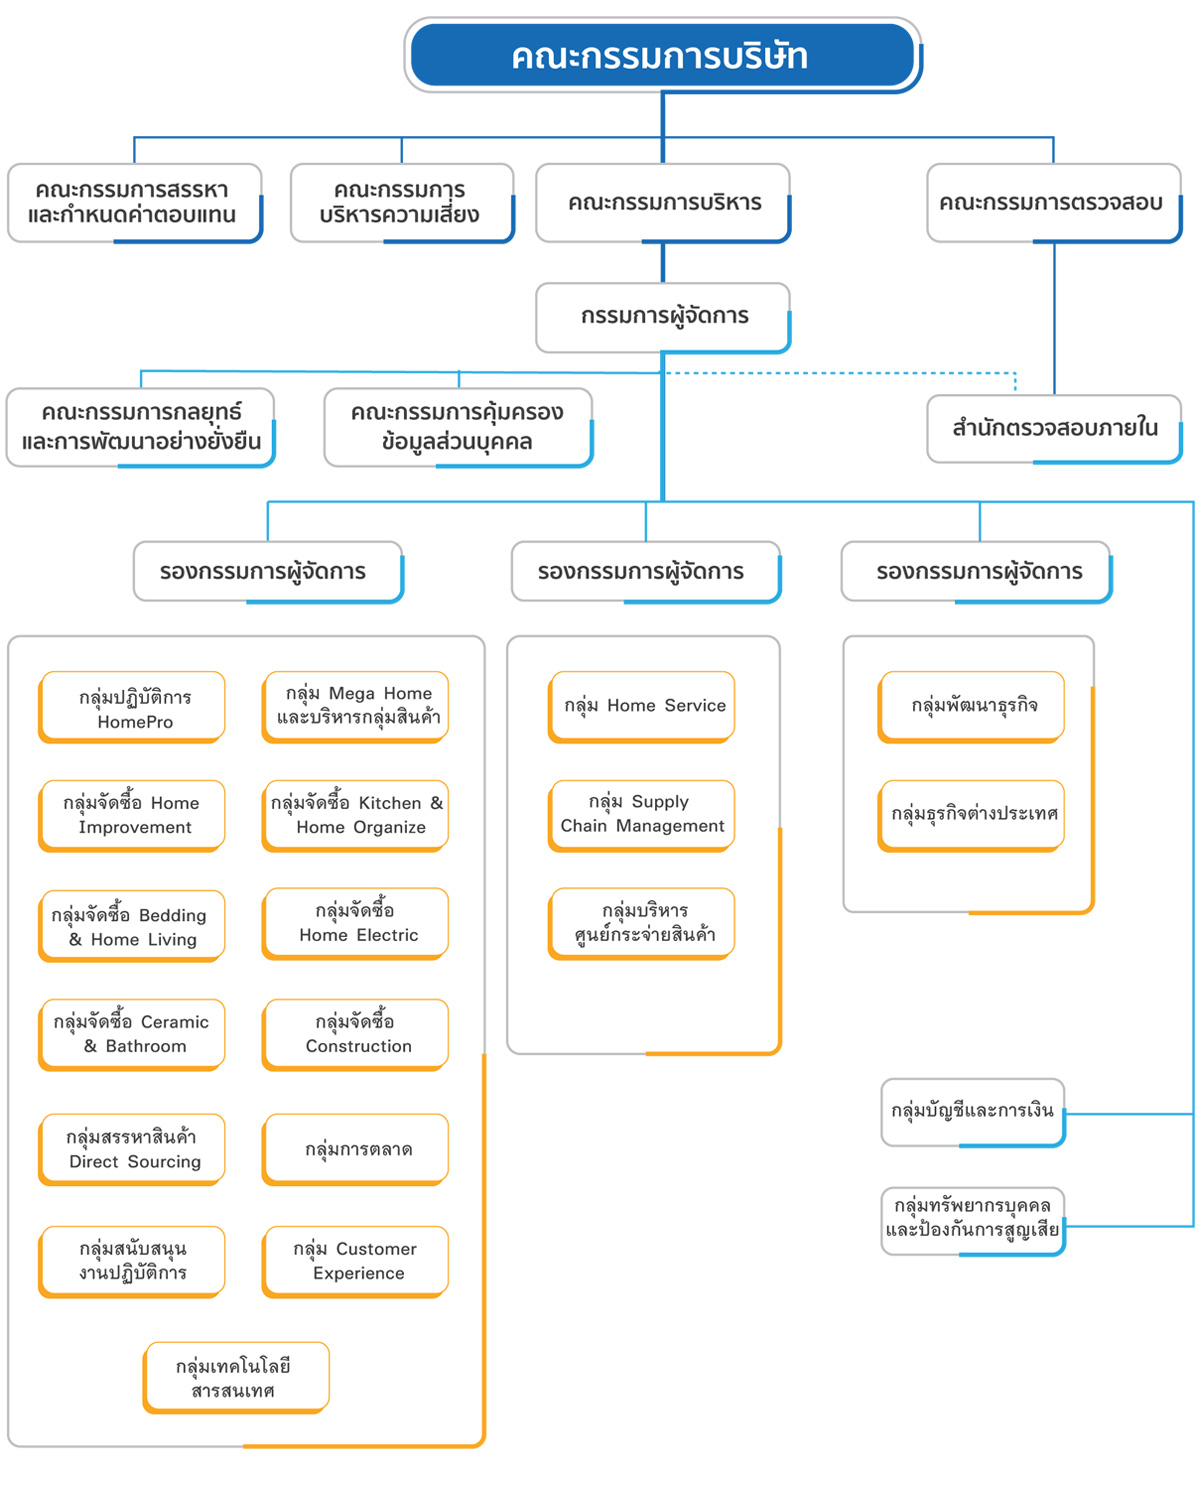
\includegraphics[width=1\textwidth]{homepro-structure}
            \caption{โครงสร้างองค์กรของ บริษัท โฮมโปรดักส์ เซ็นเตอร์ จำกัด (มหาชน)}\label{homepro-structure}
        \end{figure}

    \subsection{ตำแหน่ง และหน้าที่ของงานที่นักศึกษาได้รับมอบหมาย}
        นักศึกษาได้ทำสหกิจในตำแหน่ง PROGRAMMER มีหน้าพัฒนาชุดพัฒนาคำสั่งทดสอบแอปพลิเคชัน E-Catalog ตามเหตุการณ์ที่ผู้ใช้แอปพลิเคชันต้องเจอ และ 
        นำไปทดสอบบน AWS Device Farm อีกทั้งเป็นผู้ร่วมจัดทำคู่มือ การติดตั้งเครื่องมือในการทำพัฒนาชุดคำสั่งทดสอบอัตโนมัติ
        วิธีการสร้างพัฒนาชุดคำสั่งทดสอบอัตโนมัติ

\section{ชื่อ และตำแหน่งของพนักงานที่ปรึกษา}
    \begin{tabular}{ll}
        ชื่อ&{\Exami}\\
        ตำแหน่ง&ผู้จัดการทั่วไป\\
        แผนก&สายบริการส่งเสริมการขาย
    \end{tabular}

\section{ระยะเวลาที่ปฏิบัติงาน}
    เริ่มปฏิบัติงานสหกิจศึกษาตั้งแต่วันที่ 1 มิถุนายน พ.ศ. 2563 ถึง 30 พฤศจิกายน พ.ศ. 2563 รวมเป็นระยะเวลา 26 สัปดาห์
